%!TEX root = ../dissertation.tex
\chapter{Analisi dei requisiti}

Questo capitolo descrive i requisiti individuati per soddisfare tutti gli obiettivi definiti nel piano di lavoro.
I requisiti descrivono in modo chiaro tutte le funzionalità del sistema finale senza entrare in dettagli implementativi o vincolare l'uso di specifiche librerie o framework.


\section{Casi d'uso}
I casi d'uso riportati sono emersi nella prima settimana di lavoro, in base al piano di lavoro stabilito precedentemente e alle informazioni fornite dal responsabile aziendale. 
Questi casi d'uso forniscono una panoramica di tutte le funzionalità che dovrà avere il sistema completo.

L'unico attore è l'utente o user, ovvero colui che utilizza il sistema. Nel contesto aziendale sarà uno dei ricercatori che vuole analizzare o effettuare altre operazioni sui dati.



\subsection{Gestione dei dati}

\begin{figure} [H]
	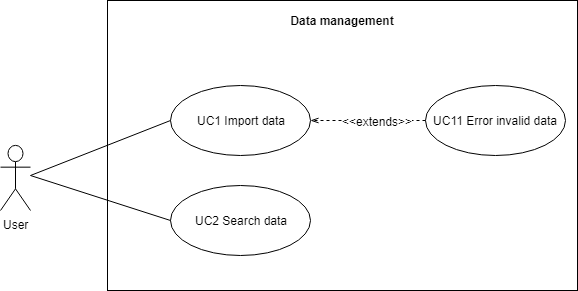
\includegraphics[width=\textwidth]{figures/UCDataManagement}
	\caption[Panoramica casi d'uso gestione dei dati]{
		Panoramica dei casi d'uso del sistema di gestione dei dati.
		\label{fig:UCDataManagement}}
\end{figure}

\begin{itemize}
	\item UC1 Import data: l'utente può importare nuovi dati nel sistema di gestione dati
	\item UC2 Search data: l'utente può cercare particolari dati in base a una condizione data, il risultato viene ritornato per poter essere analizzato in seguito
	\item UC11 Error invalid data: l'utente viene informato se i dati importati non sono nel formato corretto
\end{itemize}


\begin{figure} [H]
	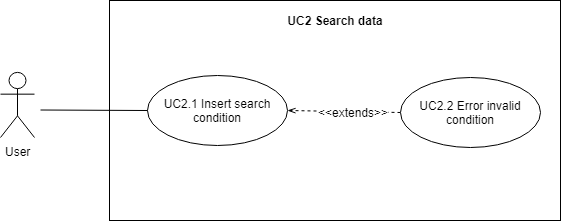
\includegraphics[width=\textwidth]{figures/UC2}
	\caption[Caso d'uso UC2]{
		Sottocasi d'uso di UC2.
		\label{fig:UC2}}
\end{figure}

\begin{itemize}
	\item UC2.1 Insert search condition: l'utente può specificare una condizione di ricerca che include uno o più dei seguenti parametri dei dati:
	\begin{itemize}
		\item \bfseries{Qgas}: Il volume della componente di gas nel flusso
		\item \bfseries{Qwater}: Il volume della componente d'acqua nel flusso
		\item \bfseries{Qwater}: Il volume della componente di petrolio nel flusso
		\item \bfseries{WLR}: Water Liquid Ratio, la percentuale di acqua sul totale del liquido
		\item \bfseries{GVF}: Gas Volume Fraction, la frazione di gas sul volume totale
		\item \bfseries{Pressure}: La pressione del flusso
		\item \bfseries{Temperature}: La temperatura del flusso
		\item \bfseries{Modules}: Quale dei moduli era installato il momento della lettura dei dati
		\item \bfseries{Time}: La data e l'orario di lettura dei dati
		\item \bfseries{Place}: Il luogo in cui sono stati letti i dati
	\end{itemize}

	\item UC2.2 Error invalid condition: l'utente viene informato se la condizione inserita non è formattata correttamente
\end{itemize}

\subsection{Analisi dei dati}


\begin{figure} [H]
	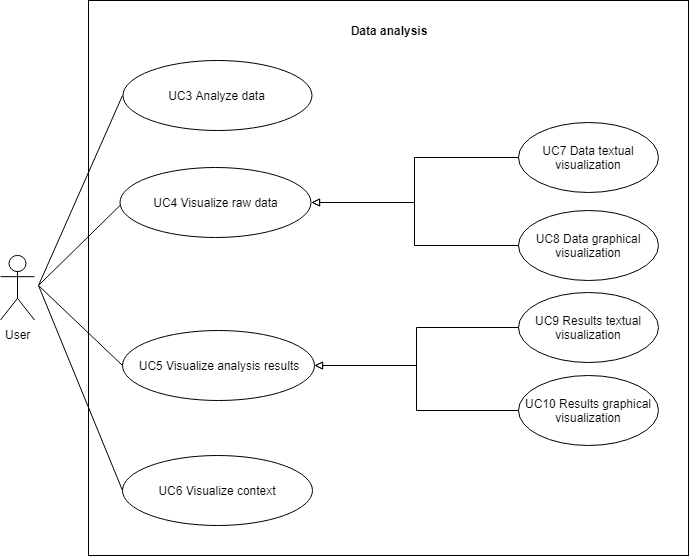
\includegraphics[width=\textwidth]{figures/UCDataAnalysis}
	\caption[Panoramica casi d'uso analisi dei dati]{
		Panoramica dei casi d'uso del sistema di analisi dei dati.
		\label{fig:UCDataAnalysis}}
\end{figure}

\begin{itemize}
	\item UC3 Analyze data: l'utente può applicare un metodo di analisi dei dati, il risultato è adatto alla visualizzazione grafica e testuale
	\item UC4 Visualize raw data: l'utente può visualizzare i dati originali
	\item UC5 Visualize analysis results: l'utente può visualizzare il risultato dell'analisi
	\item UC6 Visualize context: l'utente può accedere a tutti i documenti relativi ai dati, ad esempio file di setup, file excel di riferimento, note del laboratorio
	\item UC7 Data textual visualization: l'utente può visualizzare i dati in un formato testuale
	\item UC8 Data graphical visualization: l'utente può visualizzare i dati in un formato grafico
	\item UC9 Results textual visualization: l'utente può visualizzare i risultati dell'analisi in un formato testuale
	\item UC10 Results graphical visualization: l'utente può visualizzare i risultati dell'analisi in un formato grafico
\end{itemize}

\begin{figure} [H]
	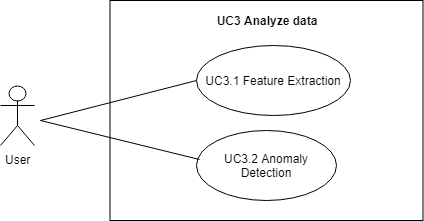
\includegraphics[width=\textwidth]{figures/UC3}
	\caption[Caso d'uso UC3]{
		Sottocasi d'uso di UC3.
		\label{fig:UC3}}
\end{figure}

\begin{itemize}
	\item UC3.1 Feature extraction: l'utente può applicare il metodo di "Feature extraction" desiderato
	\item UC3.2 Anomaly detection: l'utente può applicare il metodo di "Anomaly detection" desiderato
	
\end{itemize}

\section{Requisiti}
\subsection{Classificazione dei requisiti}
Tutti i requisiti sono classificati in base alla tipologia, alla priorità e alla fonte. Ogni requisito è inoltre associato a un codice identificativo univoco.

Le possibili tipologie sono:
\begin{itemize}
	\item GR: General Requirements, per i requisiti generali sul funzionamento
	\item SR: System Requirements, per i requisiti che riguardano le caratteristiche del sistema
	\item QR: Quality Requirements, per i requisiti di qualità
	\item DOC: Documentation, per i requisiti che riguardano la documentazione
\end{itemize}
Le possibili priorità sono:
\begin{itemize}
	\item Obbligatorio
	\item Desiderabile
	\item Opzionale
\end{itemize}
Le possibili fonti sono:
\begin{itemize}
	\item PF: Pietro Fiorentini
	\item Interno
\end{itemize}


\subsection{Requisiti generali}
\begin{table} [H]
	\centering
	\begin{tabularx}{\textwidth}{|c c X c|} 
		\hline
		ID & Priorità & Requisito & Fonte \\ [0.5ex] 
		\hline\hline
		GR-001 & Obbligatorio & L'utente può importare nuovi dati nel sistema & PF \\ 
		\hline
		GR-002 & Obbligatorio & L'utente può cercare particolari dati in base a una condizione data & PF \\ 
		\hline
		GR-003 & Desiderabile & L'utente può applicare un qualunque metodo di analisi al risultato della ricerca & PF \\ 
		\hline
		GR-004 & Obbligatorio & L'utente può applicare il metodo di feature extraction desiderato & PF \\ 
		\hline
		GR-005 & Obbligatorio & L'utente può applicare il metodo di anomaly detection desiderato & PF \\ 
		\hline
		GR-006 & Obbligatorio & L'utente può visualizzare i dati in un formato testuale & PF \\ 
		\hline
		GR-007 & Desiderabile & L'utente può visualizzare i dati in un formato grafico & PF \\ 
		\hline
		GR-008 & Obbligatorio & L'utente può visualizzare i dati risultanti da un'analisi in un formato testuale & PF \\ 
		\hline
		GR-009 & Desiderabile &L'utente può visualizzare i dati risultanti da un'analisi in un formato grafico & PF \\ 
		\hline
		GR-010 & Desiderabile & L'utente può accedere a tutti i documenti contestuali relativi ai dati ricercati & PF \\ 
		\hline
		GR-011 & Obbligatorio & Il sistema deve offrire un'interfaccia per cercare e ritornare i file richiesti & PF \\ 
		\hline
		GR-012 & Obbligatorio & Il sistema deve offrire un'interfaccia per accedere al contenuto dei file richiesti & PF \\ 
		\hline
		GR-013 & Obbligatorio & Il sistema è in grado di leggere e utilizzare il contenuto dei file BIN e BIX & PF \\ 
		\hline
		GR-014 & Opzionale & Il sistema è in grado di leggere e utilizzare il contenuto dei file txt e xls & PF \\ 
		\hline

	\end{tabularx}
	\caption{Tabella dei requisiti generali}
\end{table}


\subsection{Requisiti di sistema}
\begin{table} [H]
	\centering
	\begin{tabularx}{\textwidth}{|c c X c|} 
		\hline
		ID & Priorità & Requisito & Fonte \\ [0.5ex] 
		\hline\hline
		SR-001 & Desiderabile & Il sistema è sviluppato in Python & PF \\ 
		\hline
		SR-002 & Desiderabile & Il sistema funziona in un sistema operativo Linux & PF \\ 
		\hline
		
	\end{tabularx}
	\caption{Tabella dei requisiti di sistema}
\end{table}

\subsection{Requisiti di qualità}
\begin{table} [H]
	\centering
	\begin{tabularx}{\textwidth}{|c c X c|} 
		\hline
		ID & Priorità & Requisito & Fonte \\ [0.5ex] 
		\hline\hline
		QR-001 & Obbligatorio & Il codice segue lo stile guida definito in PEP8 & Interno \\ 
		\hline
		
	\end{tabularx}
	\caption{Tabella dei requisiti di qualità}
\end{table}

\subsection{Documentazione}
\begin{table} [H]
	\centering
	\begin{tabularx}{\textwidth}{|c c X c|} 
		\hline
		ID & Priorità & Requisito & Fonte \\ [0.5ex] 
		\hline\hline
		DOC-001 & Obbligatorio & Stesura del documento "Requirements Specification" & PF \\ 
		\hline
		DOC-002 & Obbligatorio & Stesura del documento "Data Management Design" & PF \\ 
		\hline
		DOC-003 & Obbligatorio & Stesura del documento "Data Analytics Design" & PF \\ 
		\hline
		DOC-004 & Obbligatorio & Stesura del documento "Feature Extraction Design \& Report" & PF \\ 
		\hline
		DOC-005 & Obbligatorio & Stesura del documento "Anomaly Detection Design \& Report" & PF \\ 
		\hline
	\end{tabularx}
	\caption{Tabella dei requisiti sulla documentazione}
\end{table}

